\chapter{固有时距离、克鲁斯卡尔几何与视界观察者}

施瓦西度规在视界处似乎变为奇异的。曲率却并非如此。为了区分这两种说法，我们首先去掉黑洞的整体尺度，然后用距视界的固有距离替换径向坐标。在视界附近，由此得到的几何就是写在加速坐标中的普通平直时空。一旦画出了这种几何，关于 Alice、Bob 和 Charlie 的问题就变成了关于世界线和光线的问题，而不是言辞上的悖论。

\section{将施瓦西半径缩放掉}

从带撇的坐标开始，以便稍后让重新标度后的变量带上熟悉的名称：
\begin{equation}
d\tau^2
=
\left(1-\frac{2MG}{r'}\right)dt'^2
-
\frac{dr'^2}{1-\frac{2MG}{r'}}
-
r'^2d\Omega_2^2.
\label{eq:l7-schwarzschild-dimensional}
\end{equation}
引入施瓦西半径和无量纲坐标
\begin{equation}
r_{\mathrm S}=2MG,
\qquad
r=\frac{r'}{r_{\mathrm S}},
\qquad
t=\frac{t'}{r_{\mathrm S}}.
\label{eq:l7-rescaling}
\end{equation}
我们取 \(c=1\)，因此时间和长度具有相同的单位。于是半径 \(r_{\mathrm S}\) 既是一个长度，也是与该长度相关联的光穿越时间。代入后得到
\begin{equation}
d\tau^2
=r_{\mathrm S}^2
\left[
\left(1-\frac1r\right)dt^2
-
\frac{dr^2}{1-\frac1r}
-
r^2d\Omega_2^2
\right].
\label{eq:l7-schwarzschild-rescaled}
\end{equation}
因此，所有不转动、不带电的施瓦西黑洞都具有相同的无量纲几何。改变质量改变的是乘在度规前面的那把尺子，而不是方括号中表达式的形状。这种情况就像在把每个距离都除以球的半径之后画球：同一幅图可以描述月球和地球，尽管其中一幅图上的一厘米代表不同的物理距离。

\begin{classroomqa}
\audiencequestion{度规的径向部分和角向部分各自带有什么符号？}
\lecturerresponse{在本书所用的 \(+---\) 号差下，两个空间部分都带负号。这个符号是在写表达式时当场确定的。角向因子既可以用正弦也可以用余弦，取决于极坐标是从轴量起还是从赤道量起；紧凑记号 \(d\Omega_2^2\) 避免了这一约定问题。
\lecturetimestamp{00:07:48--00:08:12}}
\end{classroomqa}

\section{视界处的曲率尺度}

这种重新标度无需冗长的张量计算就回答了一个重要的物理问题。度规分量是无量纲的。克里斯托费尔符号包含一个坐标导数，因此具有长度的倒数的量纲，而黎曼张量在物理正交归一标架中的分量具有量纲
\begin{equation}
[g_{\mu\nu}]=1,
\qquad
[\Gamma^\mu{}_{\nu\rho}]=L^{-1},
\qquad
[R_{\hat\alpha\hat\beta\hat\gamma\hat\delta}]
=L^{-2}.
\label{eq:l7-curvature-dimensions}
\end{equation}
在视界 \(r=1\) 处，唯一可用的物理长度是 \(r_{\mathrm S}\)。因此潮汐曲率尺度必定为
\begin{equation}
\left|R_{\hat\alpha\hat\beta\hat\gamma\hat\delta}\right|_{\mathrm{hor}}
\sim \frac{1}{r_{\mathrm S}^2}.
\label{eq:l7-horizon-curvature}
\end{equation}
更一般地，它是 \(r_{\mathrm S}^{-2}\) 乘以 \(r\) 的一个无量纲函数。这一陈述涉及的是黎曼潮汐场，而不是里奇标量，后者在施瓦西真空中为零。

物理结论立刻可得。增大质量会增大 \(r_{\mathrm S}\)，并减弱视界处的潮汐场。小黑洞可以在一个延展物体穿过时将其拉散；而在超大质量黑洞的视界附近，潮汐力可能很温和。然而曲率向内增长，并在 \(r=0\) 处发散。因此视界和奇点是截然不同的对象。

\section{距视界的固有时距离}

在接下来的局部计算中，令 \(r_{\mathrm S}=1\)。在相对论中，坐标变换并非表面修饰：糟糕的坐标可能把规则的几何隐藏在奇异的系数之后。施瓦西坐标差 \(r-1\) 并不是从视界量起的径向距离。

\begin{figure}[htbp]
\centering
\includegraphics[width=0.78\textwidth]{lecture_07_figure_02.png}
\caption{黑板上所用的径向坐标线。视界位于 \(r=1\)，而 \(r=0\) 是曲率奇点。}
\lectureframe{00:16:11}
\end{figure}

保持 \(t\) 和角度固定。于是正的空间线元为
\begin{equation}
ds^2=\frac{dr^2}{1-\frac1r},
\qquad
ds=\sqrt{\frac{r}{r-1}}\,dr.
\label{eq:l7-radial-proper-line}
\end{equation}
用下式定义距视界的无量纲固有时距离：
\begin{equation}
\rho(r)
=
\int_1^r\sqrt{\frac{r'}{r'-1}}\,dr'.
\label{eq:l7-rho-definition}
\end{equation}
当恢复整体尺度时，物理距离为 \(r_{\mathrm S}\rho\)。我们不需要该积分的闭式形式。我们只需要它的导数：
\begin{equation}
\frac{d\rho}{dr}
=\sqrt{\frac{r}{r-1}},
\qquad
d\rho^2
=\frac{dr^2}{1-\frac1r}.
\label{eq:l7-rho-derivative}
\end{equation}
于是复杂的径向项恰好变成 \(-d\rho^2\)。这一简化正是引入 \(\rho\) 的原因。

现在再对时间坐标作一次重新标度，
\begin{equation}
\omega=\frac{t}{2}.
\label{eq:l7-omega}
\end{equation}
由于 \(r\) 是 \(\rho\) 的函数，度规可以写成
\begin{equation}
d\tau^2
=
F(\rho)\rho^2d\omega^2
-
d\rho^2
-
r(\rho)^2d\Omega_2^2.
\label{eq:l7-rho-metric}
\end{equation}

\begin{classroomqa}
\audiencequestion{\(F(\rho)\) 是否只是为了令时间系数具有 \(F(\rho)\rho^2\) 的形式而被定义的？}
\lecturerresponse{是的。在这一点上，这种因式分解没有独立的物理内容。它是一个方便的定义。它的用处出现在取 \(F\) 在视界附近和远离视界处的极限时。
\lecturetimestamp{00:26:39--00:26:59}}
\end{classroomqa}

在远处，施瓦西时间系数趋于一。由于 \(dt=2d\omega\)，这变为
\begin{equation}
\lim_{\rho\to\infty}F(\rho)\rho^2=4.
\label{eq:l7-far-limit}
\end{equation}
在视界附近，式 ~\eqref{eq:l7-rho-definition} 给出
\begin{equation}
\begin{aligned}
\rho&\simeq 2\sqrt{r-1},\\
r(\rho)&=1+\frac{\rho^2}{4}+O(\rho^4),\\
\lim_{\rho\to0}F(\rho)&=1.
\end{aligned}
\label{eq:l7-near-expansion}
\end{equation}

\begin{figure}[htbp]
\centering
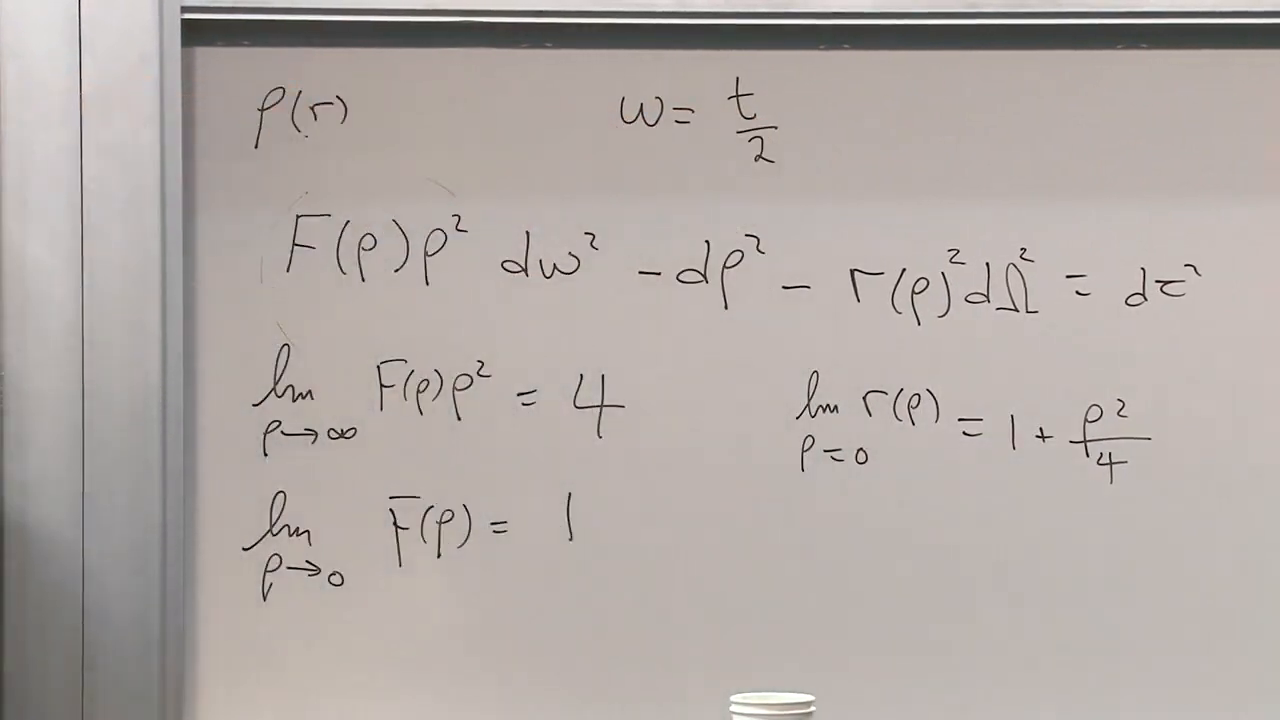
\includegraphics[width=0.90\textwidth]{lecture_07_figure_03.png}
\caption{\((\rho,\omega)\)中的度规、其渐近时间系数，以及近视界极限\(F\to1\)和\(r=1+\rho^2/4+\cdots\)。}
\lectureframe{00:37:30}
\end{figure}

\section{视界处隐藏的平直时空}

在\(\rho=0\)附近，式~\eqref{eq:l7-rho-metric}的径向-时间部分化为
\begin{equation}
d\tau_{\mathrm{radial}}^2
\simeq
\rho^2d\omega^2-d\rho^2.
\label{eq:l7-rindler-metric}
\end{equation}
这是双曲极坐标下的平直闵可夫斯基时空。定义
\begin{equation}
X=\rho\cosh\omega,
\qquad
T=\rho\sinh\omega.
\label{eq:l7-rindler-transform}
\end{equation}
于是
\begin{equation}
dT^2-dX^2
=
\rho^2d\omega^2-d\rho^2.
\label{eq:l7-minkowski-check}
\end{equation}
常\(\rho\)曲线满足
\begin{equation}
X^2-T^2=\rho^2
\label{eq:l7-constant-rho}
\end{equation}
并且是双曲线。常\(\omega\)曲线是从原点出发的射线。当\(\omega\to\infty\)时，这些射线趋近于零线\(T=X\)。因此，表面上被放逐到无限坐标时间的施瓦茨席尔德视界，在正则图中不过是一条普通的零线。

\begin{figure}[htbp]
\centering
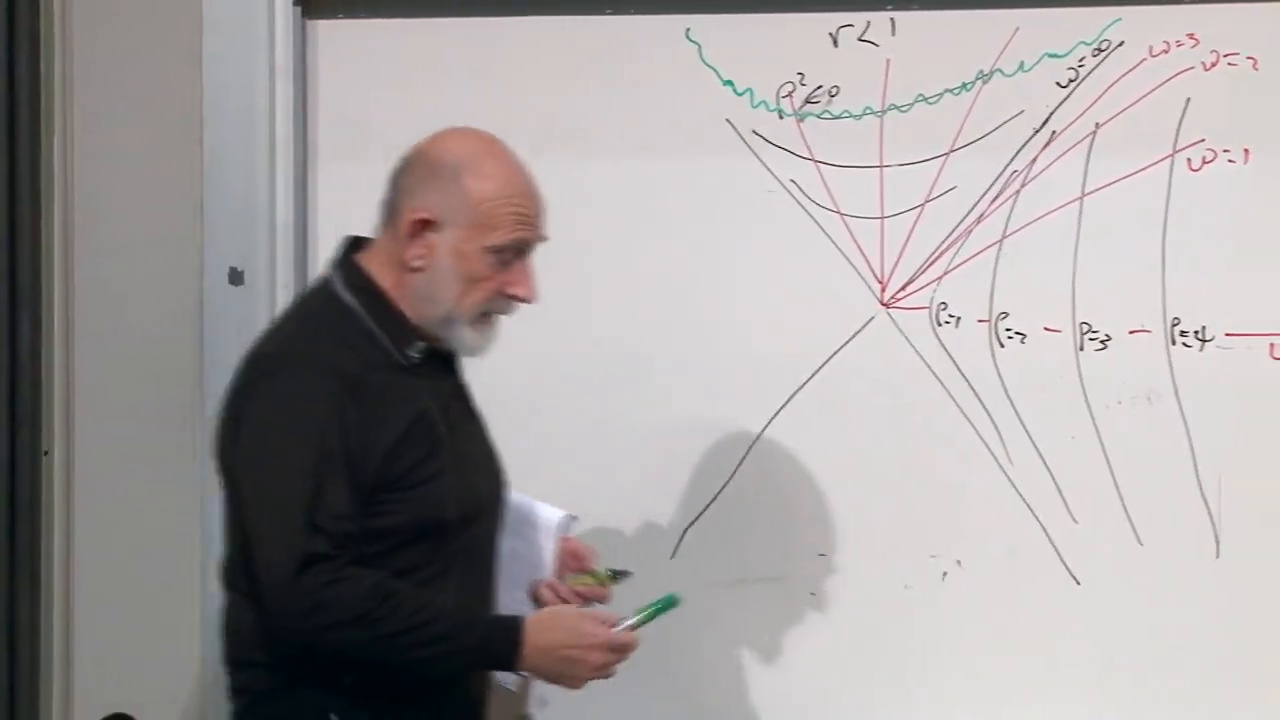
\includegraphics[width=0.88\textwidth]{lecture_07_figure_06.png}
\caption{完整的图板几何：常\(\rho\)双曲线、常\(\omega\)射线、零视界，以及其上方的\(r<1\)区域。}
\lectureframe{00:38:30}
\end{figure}

\begin{figure}[htbp]
\centering
\resizebox{0.96\linewidth}{!}{%
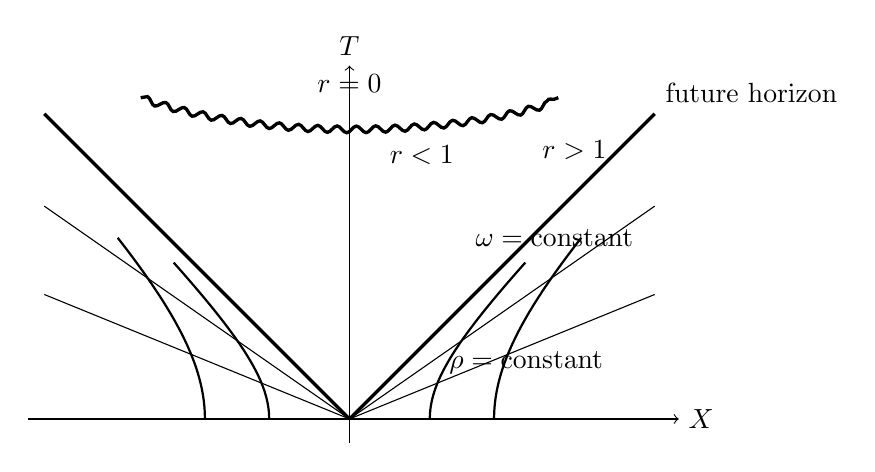
\begin{tikzpicture}[scale=1.02]
\draw[->] (-4.0,0) -- (4.1,0) node[right] {$X$};
\draw[->] (0,-0.3) -- (0,4.4) node[above] {$T$};
\draw[very thick] (0,0) -- (3.8,3.8)
  node[above right] {future horizon};
\draw[very thick] (0,0) -- (-3.8,3.8);
\draw[thick]
  plot[domain=0:1.42,samples=50]
  ({1.0*cosh(\x)},{1.0*sinh(\x)});
\draw[thick]
  plot[domain=0:1.05,samples=50]
  ({1.8*cosh(\x)},{1.8*sinh(\x)});
\draw[thick]
  plot[domain=0:1.42,samples=50]
  ({-1.0*cosh(\x)},{1.0*sinh(\x)});
\draw[thick]
  plot[domain=0:1.05,samples=50]
  ({-1.8*cosh(\x)},{1.8*sinh(\x)});
\draw[thin] (0,0) -- (3.8,1.55);
\draw[thin] (0,0) -- (3.8,2.65);
\draw[thin] (0,0) -- (-3.8,1.55);
\draw[thin] (0,0) -- (-3.8,2.65);
\draw[very thick,decorate,decoration={snake,amplitude=1.2pt,segment length=7pt}]
  (-2.6,4.0) .. controls (-1.2,3.5) and (1.2,3.5) .. (2.6,4.0);
\node at (0,4.18) {$r=0$};
\node at (2.2,0.7) {$\rho=\mathrm{constant}$};
\node at (2.55,2.25) {$\omega=\mathrm{constant}$};
\node at (0.9,3.28) {$r<1$};
\node at (2.8,3.35) {$r>1$};
\end{tikzpicture}
}
\caption{一个清晰的因果重构。视界是一条零线，而曲率奇点\(r=0\)是洞内的未来边界。}
\label{fig:l7-kruskal-clean}
\end{figure}

小\(\rho\)极限不同于欧几里得极坐标中的小半径极限。一个小的欧几里得圆收缩为一点。一条常\(\rho\)双曲线则趋近于整条零线。因此，\(\rho=0\)标记的是整个视界，而不仅仅是两轴的交点。

外部公式可以解析延拓到\(r<1\)。在视界附近，\(r-1\simeq\rho^2/4\)，因此内部在形式上对应于\(\rho^2<0\)。人们可以把\(\rho\)称为虚的，但更干净的做法是使用\(\rho^2\)、\(r\)或正则坐标\(T,X\)。施瓦茨席尔德\(t\)和\(r\)系数的符号在内部互换。这并不意味着物理手表变成了尺子。它意味着施瓦茨席尔德坐标交换了它们的因果性质。

\begin{classroomqa}
\audiencequestion{视界内部的水平双曲线是什么，直线射线又是什么？}
\lecturerresponse{双曲线是常\(r\)，等价地常\(\rho^2\)，延拓到\(r<1\)中。射线是常施瓦茨席尔德时间。在外部它们构成有用的坐标网格；在内部，同样的标记不可被误认为物理观测者的轨迹。
\lecturetimestamp{00:44:12--00:44:59}}
\end{classroomqa}

\begin{classroomqa}
\audiencequestion{竖直方向是时间坐标吗，它代表谁的参考系？}
\lecturerresponse{它是新时空图中的正则时间方向，但不是奇异的施瓦茨席尔德时间\(t\)。该图适应于自由下落的因果结构。被保持在固定外部半径处的观测者沿双曲线运动，必须加速；自由下落的观测者则平滑地穿过零视界。
\lecturetimestamp{00:45:54--00:46:48}}
\end{classroomqa}

\begin{classroomqa}
\audiencequestion{如果内部\(\rho^2<0\)，那么\(i\)的显式因子在哪里？}
\lecturerresponse{可以引入一个虚的\(\rho\)，但这样做毫无所得。不变内容由\(r\)、\(\rho^2\)以及实正则坐标\(T,X\)承载。关系\(r-1\simeq\rho^2/4\)只是近视界展开。
\lecturetimestamp{00:52:35--00:53:00}}
\end{classroomqa}

在讲义中，正则图常被描述为克鲁斯卡尔图景。严格地说，精确的克鲁斯卡尔坐标包含一个径向因子，使完整的施瓦茨席尔德度规保持正则，而式~\eqref{eq:l7-rindler-transform}是它的近视界形式。因果信息是相同的：视界是光滑的，但内部每一条未来指向的类时或零曲线都终止于\(r=0\)。任何超光速转向都不能把它带回穿过视界。

\subsection{坐标奇异性是如何被理解的}

视界的光滑性在历史上难以看出，因为原来的施瓦茨席尔德坐标使其系数看起来奇异。爱丁顿以及后来的芬克尔斯坦引入了穿越视界的坐标，芬克尔斯坦识别出了单向因果边界。克鲁斯卡尔凭借从等离子体物理中获得的坐标变换才能，为永恒解提供了全局正则图景。

讲座随后在约翰·惠勒（John Wheeler）处稍作停留，正是他帮助使“黑洞”这一说法变得无法回避。这一停留既是个人性的，也是历史性的：即便在包括关于核竞赛的判断在内的政治判断上存在尖锐分歧，惠勒仍被铭记为一位温和而深思的朋友。讲座提供了一个幽默的个人轶事，以抵制将惠勒刻画为在社会习俗上循规蹈矩之人的漫画式形象。技术要点则在“黑洞无毛”这一反驳中重新出现。一个受到扰动的非旋转黑洞会迅速趋于球对称；一个旋转的黑洞则趋于由其守恒参数所固定的定常形状。这是讲座对无毛思想的定性版本，而不是对完整定理的证明。

\section{爱丽丝穿越；鲍勃留在外面}

最大延拓图包含一些区域，这些区域并不出现在由普通初始数据坍缩而成的恒星的简单时空中。对于观察者实验，我们只使用外部、未来视界和黑洞内部。

\begin{figure}[htbp]
\centering
\includegraphics[width=0.84\textwidth]{lecture_07_figure_04.png}
\caption{爱丽丝的下落世界线以及常施瓦西时间光线。极限光线标记为\(t=\infty\)。}
\lectureframe{00:54:54}
\end{figure}

爱丽丝自由下落。她的世界线穿过视界，并在有限的固有时内到达奇点。如果黑洞足够大，使得那里的潮汐力很小，那么在她穿过视界时，她的时钟不会发生任何奇异的事情。

鲍勃则留在固定的外部半径处。保持位置需要加速度。来自爱丽丝轨迹上较后各点的光，会以越来越长的延迟和越来越大的红移到达他那里。在施瓦西时间中，爱丽丝趋近\(t=\infty\)，而鲍勃永远不会接收到她穿过视界之后发出的信号。这些是关于因果信号和外部切片的陈述，而不是视界处存在物质表面的证据。

\begin{classroomqa}
\audiencequestion{如果鲍勃看到爱丽丝变慢，爱丽丝是否必然看到鲍勃变快？}
\lecturerresponse{不会。在她的世界线存续期间，爱丽丝继续接收到来自鲍勃的普通光信号。鲍勃的世界线上存在一个能够到达她的最后事件，但那个事件之所以是最后的，只是因为爱丽丝随后撞上了奇点。鲍勃身上没有发生任何突然的事情。观测总是看向过去光锥，而这两条世界线具有不对称的因果关系。
\lecturetimestamp{00:58:31--01:01:23}}
\end{classroomqa}

\begin{classroomqa}
\audiencequestion{如果鲍勃知道，在他的坐标中爱丽丝仍然靠近视界，他能否下去把她救回来并返回？}
\lecturerresponse{一条救援世界线必须在爱丽丝穿过事件视界之前与她相遇。在那个事件之后，没有任何未来指向的路径能够与她相遇并返回外部。施瓦西切片把穿越放在\(t=\infty\)这一事实，并不会让爱丽丝停留在一个可被救回的物质表面上；它表明，这些切片并不提供跨越视界的全局“现在”概念。
\lecturetimestamp{01:01:24--01:02:12}}
\end{classroomqa}

\section{查理跟随爱丽丝}

让查理在爱丽丝身后不远处下落。于是两人在视界附近都近似处于惯性运动。他们可以交换信号、双向交谈，甚至手拉手。两人都找不到标记视界的路标。与鲍勃的对比并不是三个有名有姓的人之间的对比。它是自由下落与一条留在外部的加速世界线之间的对比。

\begin{classroomqa}
\audiencequestion{如果爱丽丝先下落，查理随后跟上，就像篮球跟着篮筐一样，鲍勃会看到什么？}
\lecturerresponse{鲍勃看到两人都趋近视界。爱丽丝因为在前方，首先显得逐渐变慢并在径向上被压缩。查理在她身后显得越来越近，但在鲍勃的极限外部视角中永远追不上她。这种视觉上的堆积并不描述任一自由下落者所感受到的东西。
\lecturetimestamp{01:04:12--01:06:05}}
\end{classroomqa}

\begin{classroomqa}
\audiencequestion{这种表观上的压平是否与潮汐力相矛盾？潮汐力应当在径向上拉伸自由下落者。}
\lecturerresponse{它们是不同的效应。压平属于鲍勃的施瓦西坐标描述。潮汐拉伸是一种局部曲率效应，爱丽丝和查理能够感受到。观察者讨论假设黑洞足够大，或者观察者足够小，以至于视界处的潮汐效应可以忽略。一个大致为太阳质量的黑洞则会在视界处具有猛烈的潮汐，而一个超大质量黑洞则可以有微弱的视界潮汐。
\lecturetimestamp{01:06:07--01:08:18}}
\end{classroomqa}

\begin{classroomqa}
\audiencequestion{当查理还位于外部时，他能看到艾丽丝穿越吗？}
\lecturerresponse{画出零射线。在艾丽丝穿越处发出的光沿视界传播，并在查理穿越时到达查理。在那个事件处，他可以计算出自己已经看到了她的穿越，尽管两位观测者都没有遇到局域的标记。此后他可以看到她位于内部。如果他在穿越之前加速离开，并成功留在外部，那么他永远不会看到那次穿越。
\lecturetimestamp{01:08:19--01:11:11}}
\end{classroomqa}

\begin{classroomqa}
\audiencequestion{如果艾丽丝已经在内部而查理在外部，他们后来的半径和穿越时间如何比较？}
\lecturerresponse{不存在一个与观测者无关的同时性关系，可以从诸如“在同一时间”这样的说法中读出来。艾丽丝在她的过去光锥上看到查理，并且只有当她自己更深入内部时，才能看到查理后来的穿越。具体的世界线和零射线回答了这个问题。要推广到许多相距很远的自由下落者，必须通过画出他们实际的因果图来检验，而不能假定存在一个普适的穿越时间。
\lecturetimestamp{01:11:14--01:12:31}}
\end{classroomqa}

在规则的近视界坐标中，自由下落轨迹几乎是一条直线。它在完整的施瓦茨席尔德几何中并不严格是直线，但在一个大的、弱弯曲的视界附近，这一近似变得很好。

\begin{classroomqa}
\audiencequestion{弦理论能否解决黑洞内部量子引力区域中发生的事情？}
\lecturerresponse{这正是问题变得微妙的地方。在奇点附近需要量子引力理论，而弦理论是一个候选框架，但相关问题当时是活跃而困难的，而不是通过简单应用经典图就能解决的。
\lecturetimestamp{01:13:04--01:13:38}}
\end{classroomqa}

\begin{classroomqa}
\audiencequestion{当艾丽丝穿越时，她自己的时钟和速度会发生什么？}
\lecturerresponse{她的时钟以其通常的局域速率继续滴答，并记录有限的固有时。在她的瞬时静止系中，她处于静止；相对于一个局域自由下落系，她具有通常的有限速度。在一个大的视界附近，几何几乎是平坦的，因此沿她的世界线的等固有时标记保持规则，直到在奇点附近曲率变得很强。
\lecturetimestamp{01:13:39--01:14:44}}
\end{classroomqa}

\begin{classroomqa}
\audiencequestion{如果鲍勃向外加速，但力度不够大，不足以避免掉进去，那会怎样？}
\lecturerresponse{那么他的世界线向外弯曲，但仍然穿过视界。如果他穿越得很晚，他可以在艾丽丝穿越后不久看到她，但他在奇点之前剩余的固有时很短。草图上的世界线斜率不是校准过的尺子或时钟；存活下来的是因果顺序，而不是画出的欧几里得长度。
\lecturetimestamp{01:14:47--01:16:31}}
\end{classroomqa}

所有这些结论都假定没有信号能超过光速。讲座简要地开玩笑提到当时最近的新闻报道，称在意大利出现了似乎超光速的中微子，这是对实验计时误差的暗示，而不是相对论的例外。因果构造本身仍然受零线限制。

\begin{classroomqa}
\audiencequestion{如果艾丽丝和鲍勃携带同步时钟，而艾丽丝朝视界俯冲并返回，这些时钟能决定问题吗？}
\lecturerresponse{当他们重合时，他们可以比较时钟，但在他们的世界线分开之后，不存在唯一的远距离同步，尤其当其中一人改变运动时。画出两条世界线以及交换的零射线。那张图为任何指定的实验提供了操作性的答案。
\lecturetimestamp{01:17:34--01:18:25}}
\end{classroomqa}

\begin{figure}[htbp]
\centering
\includegraphics[width=0.86\textwidth]{lecture_07_figure_05.png}
\caption{用于回答艾丽丝、鲍勃和查理问题的累积因果图。每个观测都通过从被观测事件到观测者世界线追踪一条零射线来定位。}
\lectureframe{01:18:12}
\end{figure}

\begin{figure}[htbp]
\centering
\resizebox{0.96\linewidth}{!}{%
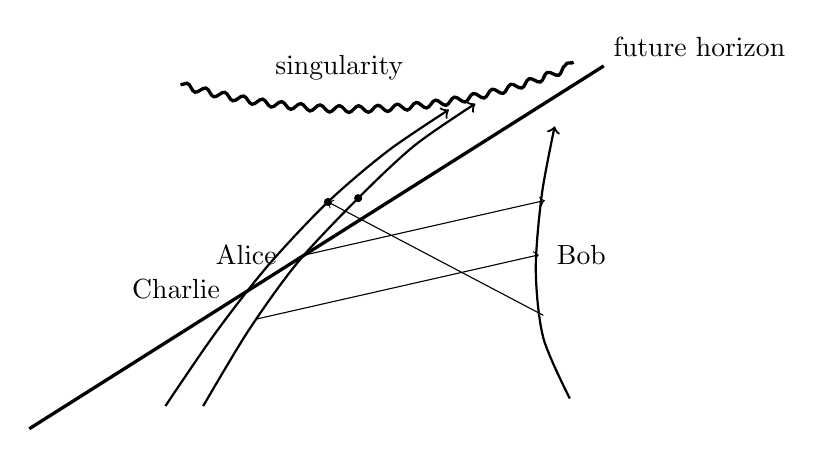
\begin{tikzpicture}[scale=0.96]
\draw[very thick] (-3.8,-0.3) -- (3.8,4.5);
\node[above right] at (3.8,4.5) {future horizon};
\draw[very thick,decorate,decoration={snake,amplitude=1.2pt,segment length=7pt}]
  (-1.8,4.25) .. controls (0.1,3.72) and (2.0,3.92) .. (3.4,4.55);
\node at (0.3,4.48) {singularity};
\draw[thick,->]
  plot[smooth] coordinates {(-1.5,0.0) (-0.9,1.0) (-0.25,1.9)
  (0.55,2.75) (1.3,3.45) (2.1,4.0)};
\node[left] at (-0.4,2.0) {Alice};
\draw[thick,->]
  plot[smooth] coordinates {(-2.0,0.0) (-1.35,0.95) (-0.65,1.85)
  (0.15,2.7) (0.95,3.38) (1.75,3.92)};
\node[left] at (-1.15,1.55) {Charlie};
\draw[thick,->]
  plot[smooth] coordinates {(3.35,0.1) (3.0,0.9) (2.9,1.8)
  (2.98,2.8) (3.15,3.7)};
\node[right] at (3.05,2.0) {Bob};
\draw[thin,->] (-0.8,1.15) -- (2.94,2.0);
\draw[thin,->] (-0.15,2.0) -- (3.02,2.72);
\draw[thin,->] (3.0,1.2) -- (0.15,2.7);
\draw[fill] (0.55,2.75) circle (1.3pt);
\draw[fill] (0.15,2.7) circle (1.3pt);
\end{tikzpicture}
}
\caption{一个示意性的观测者图。鲍勃的外部观测以及艾丽丝和查理相互之间的观测是不同的零射线构造，而不是互易时钟的口号。}
\label{fig:l7-observers-clean}
\end{figure}

\begin{classroomqa}
\audiencequestion{鲍勃是否在无限长的时间内看到艾丽丝，这是否意味着在他的现实中她永远不会死亡？}
\lecturerresponse{鲍勃在他自己时间的一个无界区间内接收到她的信号，但他看到她的时钟减慢到零速率，并且只接收到她在穿越之前发出的有限序列的心跳。“现实”一词掩盖了局域事件与观测者渐近记录之间的区别。艾丽丝在视界处并没有经历时钟停止；鲍勃的记录越来越延迟并且越来越红移。
\lecturetimestamp{01:18:32--01:20:59}}
\end{classroomqa}

\begin{classroomqa}
\audiencequestion{爱丽丝穿过视界后，会突然看到所有曾经冻结在视界上的旧物质吗？}
\lecturerresponse{不会发生突然的清除。当她下落时，她用来看到更早物质的过去光锥连续地变化。她可以推断，现在到达她这里的光是更早发出的，而那些物质在她之前穿过了视界。查理对爱丽丝的观察给出了同样的教训：两次穿越都不会产生局部的间断，也不会揭示出一堆隐藏的椅子和恐龙。
\lecturetimestamp{01:21:02--01:23:48}}
\end{classroomqa}

\begin{classroomqa}
\audiencequestion{有没有对下落者会看到什么进行逼真模拟？}
\lecturerresponse{讲座提到了安德鲁·汉密尔顿的黑洞可视化。它们可以传达入射光的严重光行差和频率移动，尽管这种显示可能与其说令人明白，不如说令人迷失方向。“视界处没有什么特别”指的是局部几何，而不是说天空看起来普通。
\lecturetimestamp{01:24:11--01:25:29}}
\end{classroomqa}

\section{从永恒黑洞到增长的黑洞}

最大延拓的永恒图的下顶点对于由恒星坍缩形成的黑洞几乎没有直接意义。在简单的坍缩几何中，只出现包含外部、未来视界和未来内部的那些部分。当允许物质改变黑洞质量时，这一区别就变得至关重要。

\begin{classroomqa}
\audiencequestion{理想化图的下顶点代表什么物理事件？}
\lecturerresponse{对于永恒的数学解，它是最大延拓的一部分。由坍缩物质形成的黑洞并不包含整个下区域。它的视界有一段形成历史，这需要不同的整体图，并将在下一讲中展开。
\lecturetimestamp{01:25:59--01:26:52}}
\end{classroomqa}

当一个小测试物体落入时，它的反作用可以忽略，固定的施瓦茨席尔德图就足够了。如果一个可观的质落入，黑洞质量和施瓦茨席尔德半径会增加：
\begin{equation}
r_{\mathrm S}=2GM,
\qquad
\Delta r_{\mathrm S}=2G\,\Delta M.
\label{eq:l7-growing-radius}
\end{equation}
视界朝着入射物体变形，视界连接起来，扭曲的共同视界迅速稳定下来。在讲座的非旋转理想化中，终点是一个稍大的球面。真实的并合还会以引力波的形式辐射能量，并且通常会留下一个旋转的黑洞。

\begin{classroomqa}
\audiencequestion{如果质量落入时视界增长，它会向外移动以迎接似乎冻结在旧视界附近的物质吗？}
\lecturerresponse{对于足够大质量的下落物体，测试粒子图像不再有效。视界变形，与入射物体的俘获区连接，并弛豫到一个更大的静止视界。事件视界的精确位置是整体性的，并且可以延伸到下落物质到达之前的一个区域。讲座有意将完整构造推迟到下一次会议。
\lecturetimestamp{01:26:55--01:29:05}}
\end{classroomqa}

\begin{classroomqa}
\audiencequestion{为什么天文学家能看到闪光，而据说物质需要无限施瓦茨席尔德时间才能到达视界？}
\lecturerresponse{明亮的辐射并非来自视界本身。吸积流或吸积盘中的气体会碰撞并在视界之外加热，包括在强光子轨道附近。那个外部等离子体可以发出到达我们这里的光。空的施瓦茨席尔德几何隔离了因果问题，但并不是天体物理环境的完整模型。
\lecturetimestamp{01:29:07--01:30:22}}
\end{classroomqa}

特征弛豫时间由光穿越时间设定：
\begin{equation}
t_{\mathrm{cross}}\sim\frac{r_{\mathrm S}}{c},
\qquad
t_{\mathrm{relax}}\sim
\text{a few to a few tens of }t_{\mathrm{cross}}.
\label{eq:l7-relaxation-scale}
\end{equation}
讲座估计\(10^{-5}\,\mathrm{s}\)为公里尺度黑洞的穿越时间，而大约\(10^{-3}\,\mathrm{s}\)为一个小并合变得几乎静止的时间。对于十亿太阳质量的黑洞，相应的时间以分钟到小时计。这些是标度估计，不是精确的并合计算。几何序列才是要点：哑铃形、花生形、近球形、静止。

\begin{classroomqa}
\audiencequestion{一个扭曲的或新并合的视界稳定下来有多快？}
\lecturerresponse{在并不比光穿过黑洞所需时间长得多的时间尺度上。因为每个长度和时间都随\(r_{\mathrm S}\)缩放，小黑洞在几分之一秒内稳定，而超大质量黑洞则在长得多的时钟时间上稳定。无毛陈述描述的是静止终点；瞬态变形通过引力辐射带走能量。
\lecturetimestamp{01:30:26--01:33:18}}
\end{classroomqa}

\begin{classroomqa}
\audiencequestion{如果在旧视界与新视界之间存在更早的物质，而另一个重物体又落入其中，Bob会看到什么？}
\lecturerresponse{把两个静态Schwarzschild图拼接在一起，无法一致地回答这个问题。必须求解或构造依赖于时间的坍缩几何，并确定其整体视界。本讲保留这个问题，并明确将答案推迟到下一周，届时主题正是视界的形成。
\lecturetimestamp{01:33:20--01:35:41}}
\end{classroomqa}

\section{尺度改变时什么会改变？}

当\(r_{\mathrm S}\)改变时，无量纲图并不改变。但图中画出的间隔的物理含义会改变：
\begin{equation}
d\tau_{\mathrm{physical}}^2
=
r_{\mathrm S}^2\,d\hat{\tau}^2,
\qquad
\ell_{\mathrm{physical}}
=
r_{\mathrm S}\,\hat{\ell}.
\label{eq:l7-scale-restoration}
\end{equation}
对于公里尺度的黑洞，代表半公里的无量纲间隔，对于大十亿倍的黑洞，代表大约五亿公里。与等大画出的球面的类比又回来了：形状不变，而一条线所代表的米尺数目随半径成比例缩放。

\begin{classroomqa}
\audiencequestion{当Schwarzschild半径改变时，因果图如何改变？}
\lecturerresponse{在半径被缩放掉之后，它并不改变。赋予该图的每个物理长度和时间都乘以\(r_{\mathrm S}\)，而相应无量纲点处的曲率则乘以\(r_{\mathrm S}^{-2}\)。
\lecturetimestamp{01:35:41--01:38:10}}
\end{classroomqa}

\begin{classroomqa}
\audiencequestion{如果Bob不是悬停在某个角位置，而是沿轨道运动，因果结论会改变吗？}
\lecturerresponse{详细的红移和到达方向会变得更复杂，但视界的因果分离不会改变。没有任何外部类时轨道能接收到从视界内部发出的信号。
\lecturetimestamp{01:38:12--01:38:26}}
\end{classroomqa}

\begin{classroomqa}
\audiencequestion{既然球壳内部引力消失，那么黑洞质量若分布在该表面上，视界内部引力是否也会消失？}
\lecturerresponse{不会。事件视界并不是承载质量的物质壳层。因此Newton球壳定理并不适用于它。本讲把静态外部解与位于曲率奇点处的点源相比较，但形成过程中当前正在下落的物质需要依赖于时间的几何，这被推迟到下一讲。
\lecturetimestamp{01:38:28--01:40:41}}
\end{classroomqa}

\section{旋转与径向几何}

角动量在坍缩中存留下来。旋转黑洞的外部几何不同于Schwarzschild：其稳态解是Kerr，旋转使视界几何发生畸变，参考系拖曳带着惯性方向绕黑洞转动。原则上，角动量是通过这些外部引力效应来测量的。具有角动量的物质不会仅仅因为穿过视界就失去它。

\begin{classroomqa}
\audiencequestion{黑洞能有可测量的角动量吗？旋转会改变其外部引力吗？}
\lecturerresponse{能。角动量作为守恒参数保留下来，使稳态几何发生形变，并产生参考系拖曳。视界不再是简单的球对称Schwarzschild视界。本讲把这种畸变定性地与地球的扁球形相比较，同时指出完整的旋转解要复杂得多。
\lecturetimestamp{01:40:45--01:42:36}}
\end{classroomqa}

\begin{classroomqa}
\audiencequestion{\(r\)与固有距离\(\rho\)之间的关系，是否意味着引力使空间收缩？}
\lecturerresponse{固有径向距离\(\rho\)满足
\begin{equation*}
\frac{d\rho}{dr}=\sqrt{\frac{r}{r-1}}>1
\end{equation*}
在单位视界之外。因此，给定的坐标增量\(dr\)在视界附近对应于更大的固有径向间隔。说空间是收缩还是拉伸，取决于所比较的是哪些坐标间隔。不变的说法就是固有距离关系本身。
\lecturetimestamp{01:42:36--01:43:20}}
\end{classroomqa}

\section{最后的问题}

\begin{classroomqa}
\audiencequestion{从Bob的观点看，Alice的钟趋近于停止。从Alice的观点看，Bob的空间或时间会终结吗？}
\lecturerresponse{不会。Alice会看到来自Bob世界线上相继事件的普通信号，直到她自己的世界线终结。她看不到Bob更晚的事件，是因为她的世界线上不存在更晚的点，而不是因为Bob或他的空间消失了。在这些规则的因果坐标中，径向零射线被画成直线；它们在另一个坐标系中表现为弯曲路径，并不改变它们连接的是哪些事件。
\lecturetimestamp{01:43:21--01:45:20}}
\end{classroomqa}

广义相对论提出两项互补的任务。给定度规，人们可以追踪测地线和零射线，以确定观测者测量到什么。给定物质分布，人们必须求解Einstein方程以求出度规。第一项任务占据了本讲。第二项通常更难，尽管对称坍缩提供了可处理的例子。

\begin{classroomqa}
\audiencequestion{蒸发中的黑洞，其视界与奇点会发生什么？}
\lecturerresponse{讲座给出了一幅示意性图景：视界收缩，并与奇异区域的端点相遇。蒸发是一个半经典量子过程，最终的普朗克尺度端点并不能由经典施瓦西图景来确定。因此，收缩的草图应被理解为定性的预览，而不是完整的量子几何。\lecturetimestamp{01:46:04--01:46:32}}
\end{classroomqa}

几乎每一个天体物理黑洞都应当旋转。恒星本身就具有角动量，而坍缩会以滑冰者收拢手臂那种熟悉的方式放大其角速度。克尔黑洞的奇异结构并不是这里画出的施瓦西\(r=0\)面，也不应被描述为物质真的以无限线速度旋转。

\begin{classroomqa}
\audiencequestion{不旋转的宏观黑洞常见吗？黑洞有多少个？}
\lecturerresponse{角动量恰好为零将是一种例外的理想化。讲座对宇宙中的黑洞总数只给出了课堂上的数量级猜测，介于星系数量与恒星数量之间，也许约为\(10^{15}\)。那是讲座时代的估计，而不是实测的普查结果。可靠的一点是，坍缩通常会保留并放大一定的角动量。
\lecturetimestamp{01:46:32--01:48:42}}
\end{classroomqa}

\begin{classroomqa}
\audiencequestion{黑洞是由已有物质形成的，还是通过量子过程出现的？}
\lecturerresponse{普通的天体物理黑洞是在已有的恒星物质坍缩时形成的。核燃烧和能量的向外流动有助于支撑恒星。当燃料耗尽时，残余物会收缩。取决于其质量和可用的压强支撑，它可能成为白矮星、中子星，或者，如果没有任何支撑能阻止坍缩，就会进入自身的施瓦西半径之内并形成黑洞。
\lecturetimestamp{01:48:43--01:50:23}}
\end{classroomqa}

\begin{classroomqa}
\audiencequestion{微观黑洞能形成吗？什么决定它们的寿命和最小尺寸？}
\lecturerresponse{这部分是推测性的。霍金蒸发对于质量越小者越快，其寿命大致按\(M^3\)标度。讲座用一座山的质量作比较，来说明一个寿命可能达到宇宙学尺度的黑洞；这个数值类比只是粗略的。早期宇宙中剧烈的密度涨落，或者能量足够高的碰撞，都是可以设想的形成机制。接近普朗克质量、约为\(10^{-5}\,\mathrm{g}\)的黑洞，标志着经典几何描述不再可信的尺度。在普通加速器中达到那样的能量，按直接的推断将需要一台大得难以置信的机器，尽管这种形成在原则上是有可能的。
\lecturetimestamp{01:50:23--01:53:31}}
\end{classroomqa}

\begin{classroomqa}
\audiencequestion{这门课程会讲到宇宙学、暗物质、暗能量、熵和引力波吗？}
\lecturerresponse{宇宙学应用，也许还有引力波，仍是以后可能涉及的主题。黑洞熵则推迟到本季度之后。讲座最后承认，那天晚上只讲完了计划材料的大约四分之一：仔细解决这些问题，比匆匆赶完大纲更重要。
\lecturetimestamp{01:53:33--01:54:38}}
\end{classroomqa}

这条操作规则经受住了在场提出的每一个问题。指定世界线，画出零射线，并确定它们所连接的事件。视界并不是局部物理失效的地方；它是这样一条边界：越过它之后，每一个指向未来的信号都留在内部。下一讲将用坍缩的源取代永恒的背景，并展示这条边界是如何形成的。
